\subsection{Tellerfedern \hfill ME}
\begin{footnotesize}
    \begin{center}
        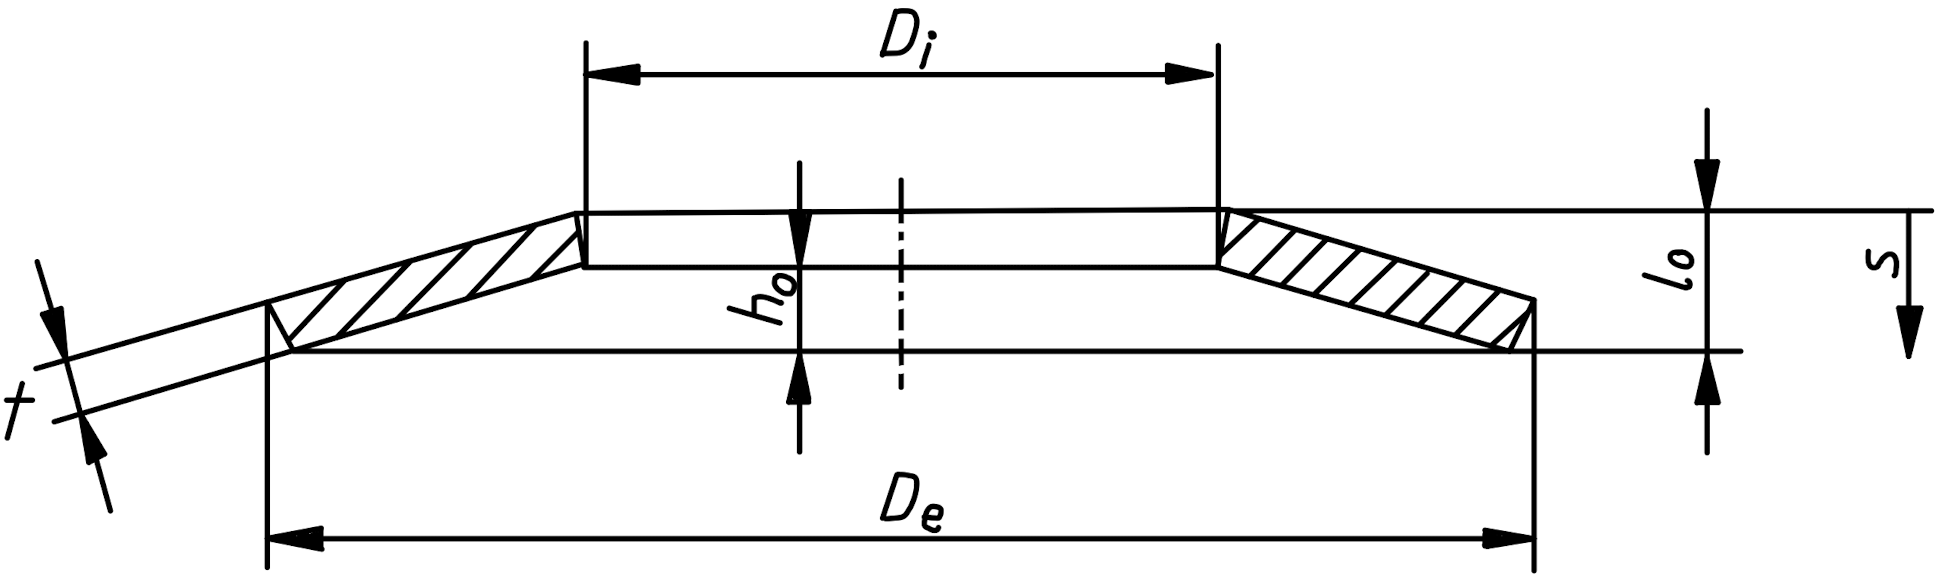
\includegraphics[width = 0.7\linewidth]{MAEIP_Tellerfeder}
        \begin{minipage}{0.5\linewidth}
            \begin{scriptsize}
                    \begin{tabular}{|c|c|c|}
                    \hline
                    Reihe & $\frac{h_0}{t}$ & Kennlinie\\
                    \hline
                    A & 0.4 & Linear\\
                    \hline
                    B & 0.75 & Mässig degressiv\\
                    \hline
                    C & 1.3 & Stark degressiv\\
                    \hline
                \end{tabular}
            \end{scriptsize}
        \end{minipage}
        \begin{minipage}{0.48\linewidth}
            \vspace{2mm}
            \frame{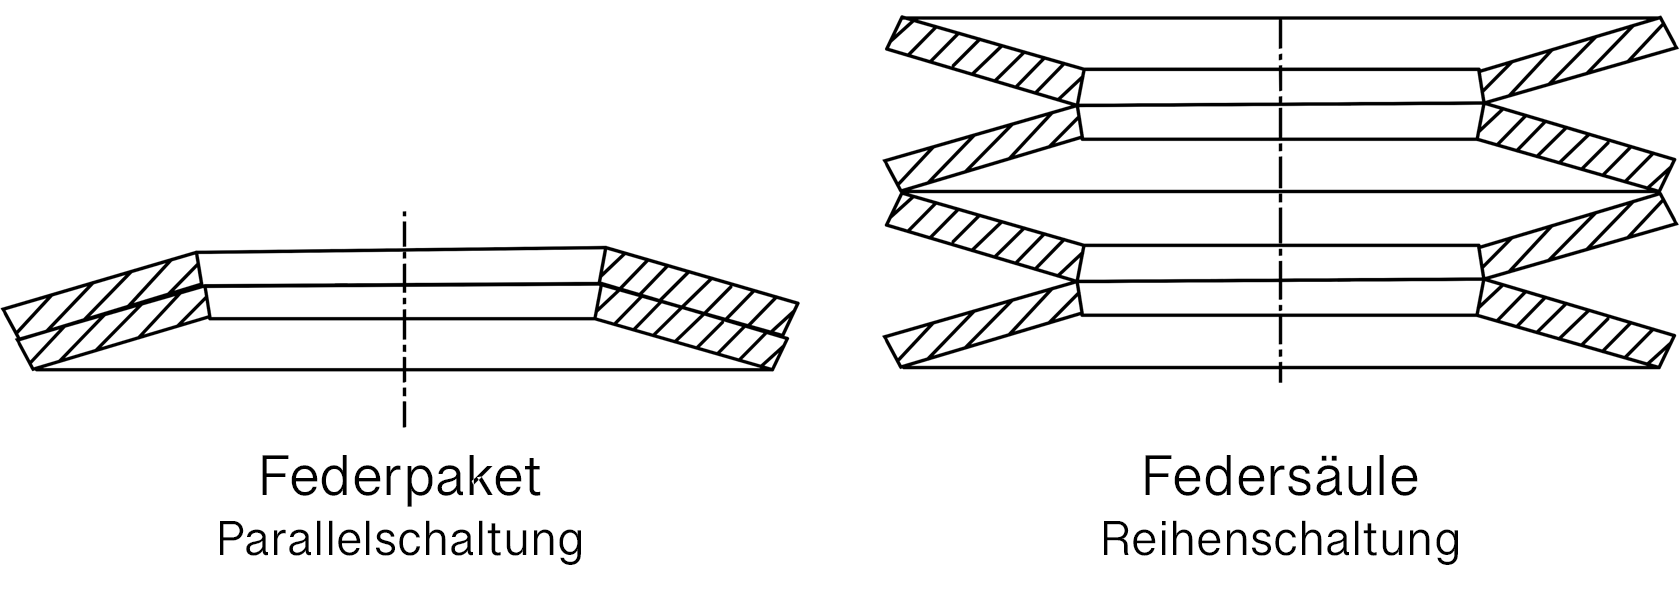
\includegraphics[width = 1.0\linewidth]{MAEIP_Federpaket}}
        \end{minipage}
        \par \vspace{2mm}
            \begin{scriptsize}
                \textbf{Federsäule:} Reihenschaltung (vgl. 8.2) / \textbf{Federpaket:} Parallelschaltung (vgl. 8.2)
            \end{scriptsize}
    \end{center}
\end{footnotesize}